\chapter{Background}\label{Introduction}

\section{Relational Databases}\label{theory}

In this chapter I give a short overview about aspects from the area of (relational) database systems that are relevant to my thesis. I introduce the relational data model and its Structured Query Language (SQL). All explanations target PostgreSQL 10.6 as state-of-the-art Database Management System (DBMS).

PostgreSQL 10.6 is used throughout this thesis as RDBMS and SQL-dialect. Its first version was developed as "POSTGRES" at Berkely 1986 \cite[xxxvi ff.]{psql}. It had its first open source release under the name "Postgres95" in 1995 where the own query language PostQUEL was replaced by SQL. As of 1997 and version 6.0 the software is named "PostgreSQL" to reflect its SQL-capabilities \cite[xxxvi ff.]{psql}.

PostgreSQL claims to be "the most advanced open-source database available anywhere" \cite[xxxvii]{psql}. It conforms to most parts of Core SQL:2011 \cite[S. 2198]{psql} and offers great extensibility and introspection. User defined functions, types, operators, index methods, statistics for the planner, procedural languages, foreign data wrappers and rewrite rules are possible. 

\subsection{Relational Data Model}
An integral part of many applications is to retrieve, modify and persist data. Depending on the complexity of the data (eg. plain key-value, hierarchical structured, associations to other data, etc.) and the requirements to the storage system (performance, query capabilities, robustness, multi-user capability, etc.) a number of solutions are viable. Relational Database Management Systems (RDBMS) are a very popular and advanced solution to manage vast amounts of interconnected data efficiently.

The original relational data model dates back to 1970 where E. F. Codd proposes a representation of data in set-theoretic \textit{relations} \cite{codd}. A relation is similar to \textit{table} with named and typed \textit{columns}. An instance of a relation is a set of tuples from the \textit{domain} of each of the columns. A subset of columns in a relation may form a unique \textit{primary key} for each of its tuples that can be included in other tables as \textit{foreign key} to establish references. A relational data model should be normalized to remove redundancies and enforce atomacity.

An important innovation by the relational model was the claim that access of the stored data should be separated from its internal (physical) representation and should be able to change without affecting the logical representation that is used by a program (\textit{data independence}). Instead of manually accessing the physical stored data, the programmer should just use a "data base sublanguage" (Codd) to specify tasks on the logical level, and the DBMS finds automatically an efficient way to perform the task on a physical level \cite[p. 3 ff.]{FoD}.

Based on Codds proposal of a "universal data sublanguage" to define and manipulate a relational model, Chamberlin and Boyce designed a "Structured English Query Language" (SEQUEL) \cite{sequel, sequel2}. The name alone highlights its declarative nature: Say \textit{what} you want, just in simple English. SEQUEL was later renamed to SQL and first standardized in 1987 as SQL:86 (ISO 9075:1987), the latest version to date is SQL:2016 (ISO/IEC 9075:2016). For this thesis, only a subset of the \textit{Data Manipulation Language} (DML) is of interest, namely reading queries.

\subsection{SQL and query evaluation}

Due to their declarative nature, SQL-Queries are no executable programs by themselves. To create an program from the query (a \textit{plan}), it is first parsed into an \textit{Abstract Syntax Tree} (AST, \autoref{fig:fib_ast}). An AST encodes the syntactic structure of the query into the structure of the AST, preserving its semantics. Parsing text into an AST is a standard step in compilation because ASTs are much more suitable to work with \cite[p. 5]{dragenbook}.

\begin{figure}[h!]
    \centering\footnotesize
    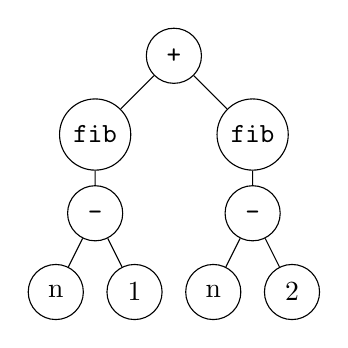
\begin{tikzpicture}[level distance=1cm,level 1/.style={sibling distance=2cm},level 2/.style={sibling distance=1cm}, every node/.style = {shape=circle, draw, align=center, minimum width=7mm, minimum height=7mm}]]
    \node {\texttt{+}}
        child { node{\texttt{fib}}
            child { node {\texttt{-}}
                child { node {n} }
                child { node {1} }
            }
        }
        child { node{\texttt{fib}}
            child { node {\texttt{-}}
                child { node {n} }
                child { node {2} }
            }
        };
    \end{tikzpicture}
    \caption{AST of \texttt{fib(n-1) + fib(n-2)}}
    \label{fig:fib_ast}
\end{figure}

The \textit{parse-tree} of the input query is transformed into a \textit{query-tree}. The transformation to the query-tree includes some desugering like expanding \texttt{T.*} to an explicit column-list, adding default \texttt{ELSE NULL} to \texttt{CASE}-statements and expanding row-comparisons \texttt{(1, 2) = (1, 4)} to boolean conjunctions \texttt{1=1 AND 1=4}. This makes it easier for the query planner to analyze the structure of the query and derive an efficient plan. Finally the query is rewritten, which primary replaces references to views by their original queries. \cite{}

The preprocessed and rewritten query is then fed into the \textit{query planner} to compile the declarative query into an procedural program (a \textit{plan-tree}) executable by the \textit{executor}. Its main responsibility is to find the fastest way to access and join the involved tables. Every (nontrivial) plan has table scans at its leafs. There are multiple ways to scan a table depending on the presence of predicates and auxiliary datastructures (\textit{indices}). Consider the query \texttt{SELECT * FROM T WHERE T.v = 5}. Depending on the size of \texttt{T} and the number of occurrences of \texttt{5} in the column \texttt{T.v} it may be most efficient to do a full \textit{sequential scan} of the entire table, filtering out rows not matching the predicate. If the table is large and there are only few rows with \texttt{T.v = 5}, an \textit{index-scan} may be much faster. With few I/O-operations the matching rows can be selectively retrieved, without reading the entire table. Various statistics are maintained to help the planner estimate the cost for each operation and choose the cheapest plan. \cite[p. 1887]{psql}


Tables in the \texttt{FROM}-clause can be combined (\textit{joined}) by different algorithms. Each algorithm has its own preconditions, strengths and weaknesses, so the choice of the appropriate join-strategy is very important. As each join-algorithm expects exactly two input tables, joining multiple tables results in a binary join-tree. The join order can impact the query performance dramatically as it determines the size of the intermediate join-results. Three tables R, S, T can either be joined as $(R \bowtie S) \bowtie T$ or as $R \bowtie (S \bowtie T)$. In general it is beneficial to choose the option that removes most rows from the result early to avoid investing time in joining rows that are eventually removed. The planner tries to attach predicates from the query to the joins to reduce the size of the join result (\textit{predicate push-down}).

Further nodes in the plan are used for sorting, aggregation, combining queries and others. Obviously, there are a lot of possible plans for a single query. To find the best plan, the query planner computes all possible plans and estimates the cost of each solution based on various statistics to select the cheapest. As the search-space for the planner growths exponentially with the number of involved tables, the exhaustive search switches to a heuristic-driven optimization when a threshold is exceeded \cite[p. 2064 ff.]{psql}.


Finally, the \textit{executor} recursively executes each node of the plan just as long as required by the parent node (Volcano Iterator Model) \cite{volcano}. Thus, each operation is not necessarily performed to completion but just as long as required to return the next row. Each plan contains therefore not only an estimate for the \textit{total cost} of the node until completion, but also minimum cost to return the first row (\textit{start up cost}). In the best case, the first returned row is just the single requested row and eg. the entire remaining table scan can be omitted. Yet, some operations need to be run to completion before being able returning the first row, eg. sorting. For these cases, the start up cost equals the actual cost.




% Building the cartesian product between tables is called a \textit{join}. Even for moderate sized tables the result of a couple of joins can be astronomically large, if done naively. Imagine build the cartesian product a table \texttt{S} with 10.000 rows, \texttt{T} with 100 rows and \texttt{R} with 1.000 rows. The resulting table would have $10.000 * 100 * 1.000 = 1.000.000.000$ rows - that escalated quickly!

% They just specify \textit{what} the user wants to achieve without telling \textit{how} (declarativity \cite[p. 21]{ullman}). To understand the "problem statement" of the user, the query is parsed, checked and rewritten before fed into the query-planner.

% It is possible to output the generated parse- and query-trees to the logfiles with configuration parameters \texttt{debug\_print\_\{parse, rewritten\}} set to true. To sanitize and parse the query-tree again, I used the great library \texttt{PgQueryHauler} by Denis Hirn \cite{denis_hirn} and Peter Richter \cite{peter_richter} to parse the logs and pretty print them as SQL again.

% There may be many possible strategies to execute a query and the best solution depends on various details (physical organization, frequencies of values, auxiliary data-structures, etc. pp) that may help to find the most efficient one. The \textit{query planner} is responsible to generate an actual executable, imperative program called a \textit{plan}.

%They specify \textit{what} the user wants to achieve without requiring any information about the exact \textit{how}. A query to count the number of rows with \texttt{t=0} from a table \textit{T} does state this intent directly as \texttt{SELECT COUNT(*) FROM T WHERE t = 0}. There is no loop incrementing a counter nor any information included about the location or retrieval of the contents of \texttt{T}. The desired result is specified at a high abstraction level and the best way to compute this result is obtained automatically. This property is known as \textit{declarativity}.

% To evaluate the query, the "problem statement" (the query) needs to be translated into a concrete "plan". This translation is done by the query planner.

% But even the query planner is not the holy grail and there are queries that perform incredibly bad or are difficult to formulate in a way the query planner can find a efficient plan.

% The most frequent form of reading queries are $\textit{SELECT s_1, s_2, ..., s_n FROM T_1, T_2, ..., T_n WHERE p}$-queries (S-F-W). The cartesian product $\texttt{T_1 \times T_2 \times \dots \times T_n}$ between the tables is built and the resulting rows are filtered by the predicate \texttt{p}. Finally, the output columns in the select-list are evaluated for each row, returning the output table.
\section{Recursion in SQL}

Recursion is a fundamental concept in everyday programming as well in computability-theory. Every recursive function consists of a number of different \textit{evaluation scenarios}. Some of them cause subsequent recursive calls (\textit{recursive scenarios}) and at least one scenario causes no recursive calls at all. Otherwise, the function will never terminate. We will call nonrecursive scenarios \textit{basecases}. The programmer usually uses conditionals to direct which scenario should be evaluated. For this thesis, I assume that conditionals are given in the form of \texttt{CASE}-expressions only, to that a \textit{predicate} is stated explicitly for each scenario. One of the main task of the translation is to collect the scenarios and identify their predicates.

Recursive functions can be implemented in SQL in two ways: As User Defined Function (UDF) or as self-referential Common Table Expression (CTE) in \texttt{WITH RECURSIVE}-queries. UDFs are functions (actually procedures) as we know them: A function with a name, an argument list, a defined return type and a function body. Recursive CTEs are different, as they are no procedures with explicit arguments but self-referential queries of a specific structure.

\subsection{Recursive User Defined Functions}
Recursive functions can be created in PostgreSQL as UDFs. UDFs can be implemented in a wide range of languages but we consider only SQL-UDFs as the pure SQL approach. There is also a number of ways to specify arguments and add modifiers. For my thesis I use just simple positional arguments without any modifiers (eg. \texttt{\$1}).

\begin{figure}[h!]
    \centering
    \begin{minted}{postgresql}
CREATE FUNCTION fac(INT) RETURNS INT AS $$
SELECT CASE WHEN $1 = 1 THEN 1
            ELSE $1 * fac($1 - 1)
       END
$$ LANGUAGE SQL;

SELECT fac(10);
    \end{minted}
    \caption{Calculation of $10!$ using a a recursive UDF \texttt{fac)}.}
    \label{fig:my_label}
\end{figure}

A UDF is mostly a black box for the query planner. They have just a fixed cost assigned as a whole (default 1000 \cite[p. 1435]{psql}) and the body of every call is repeatedly planned before execution.

Under certain circumstances, PostgreSQL can optimize some function calls. Very simple functions can be inlined during planning \cite{psqlWikiUDFinlining}  (see \autoref{fig:inlining}), but this is done only once, so its impact for recursive functions is not a game-changer.


\begin{figure}[h!]
    \centering
    \begin{minted}{postgresql}
CASE WHEN ($1 = 1) THEN 1
     ELSE ($1 * CASE WHEN (($1 - 1) = 1) THEN 1
                     ELSE (($1 - 1) * fac(($1 - 1) - 1))
                END)
END
    \end{minted}
    \caption{The query-body of \texttt{fac} after the planner has inlined the call to \texttt{fac(\$n - 1)}.}
    \label{fig:inlining}
\end{figure}

Identical calls to an function marked as \texttt{IMMUTABLE} can be folded into a constant during planning \cite[p. 995]{psql}. The impact on usual queries may be significant when a call to an expensive function eg. in a where-clause is repeated for every row of a table:\\
\begin{minted}{postgresql}
SELECT * FROM T WHERE T.v IS BETWEEN fac(99) AND fac(100);
\end{minted}
Instead of evaluating \texttt{fac(99)} and \texttt{fac(100)} exactly $|T|$ times, the planner may be able to evaluate those functions once and replace the values in the where-clause with that values. For recursive SQL-UDFs, this happens as well, but isolated for each invocation of a UDF. There is nothing folded into constants across levels of recursion.

\subsection{Recursive Common Table Expressions}

Common Table Expressions (CTEs) are a convenient way to define auxiliary queries once in advance to use them similar to temporary tables in the contained query. CTEs help breaking down a big query down to smaller individual parts. CTEs are only evaluated once, which can improve performance. On the other hand, CTEs are known to be "optimization fences" as the planner does not perform predicate pushdown into CTEs.


\begin{figure}[h!]
    \centering
    \begin{minted}{postgresql}
WITH RECURSIVE T(i, v) AS (
 SELECT 1, 1
   UNION ALL
 SELECT i + 1, v * (i + 1) FROM T WHERE i < 10
)
SELECT v FROM T WHERE i = 10;
    \end{minted}
    \caption{Calculation of $10!$ using a self-referential CTE.}
    \label{fig:my_label}
\end{figure}


CTEs also exist also in a "recursive" variant, which makes SQL queries much more expressive. Actually, since the introduction of recursive CTEs in SQL:1999, queries are turing-complete. Every intuitively computable function can expressed as a SQL-query. PostgreSQL supports this feature since Version 8.4 (2009) \cite[p. 2811]{psql}. Implementations in PostgreSQL for turing-machines and cyclic tag systems exist, demonstrating this property \cite{psqlWikiCTS, psqlWikiTM}.

Yet, recursive functions need to be implemented in a special style using self-referential CTEs inside \texttt{WITH RECURSIVE}-queries. This constraints origin from the fact that they are actually evaluated iterativly. Each self-referential CTE consist of a \texttt{UNION} or \texttt{UNION ALL} that divides the starting query from the "recursive" query. The recursive query contains a reference to the CTE itself. Evaluation happens in a iterative fashion: In each iteration the self-reference points to a \textit{working table} containing the results from the previous iteration. When using the variant with \texttt{UNION}, each iteration returns only (globally) new rows. The rows from each iteration is added to the result of the CTE.

As soon as the working table is empty, evaluation stops. In the case of \texttt{UNION ALL} this happens only when an iteration returns the empty table. Using \texttt{UNION}, it stops when the iteration returns no previously unseen rows. RCTEs resembles therefore a while loop.

The semantics of a self-referential CTE using \texttt{UNION} can be summarized as follows:

$$
q_0 ~\cup ~\underbrace{q_r(q_0)}_{q_1} ~\cup~ \underbrace{q_r(q_1)}_{q_2}~ \cup~\underbrace{q_r(q_2)}_{q_3}~ \cup ~\hdots ~ \cup ~ \underbrace{q_r(q_n)}_{= \emptyset}
$$

For \texttt{UNION ALL} the set semantics need to be replaced with bag semantics to allow duplicates.

Beside the special structure of a RCTE, they come with two important restrictions. First, only a single (direct) self-reference is allowed in the self-referential query. A simple workaround is to use a CTE that "proxies" access, so this limitation is not severe.

More notably is that only the previous iteration can be referenced. This is a strong limitation as this allows only the convenient formulation of linear recursive functions. In linear recursion a single recursive call leads to a single subsequent call. To evaluate a call, only the result of the previous call is therefore required. The usual workaround is to use \texttt{UNION ALL} semantics to allow duplicates and to add the previous result to the new results. The obvious caveat of this solution is that the resulting table becomes large quickly. After $n$ iterations, the results from the first iteration is contained $n$ times, results from second iteration $n-1$ times and so on. The result table grows quadratically. Furthermore, there must be taken care of including a stopping criterion to eventually prevent include the previous rows again and instead return the empty table.


\section{Related Work}

Performing computations close to the data within the DBMS is favorable especially in situations where the data does not fit into main memory. In particular, computations for statistical and machine learning applications can profit from the scalability of RDBMs \cite{SQLforML,PCAinSQL,MLwithUDFs,MLinSQL2}.

Transforming a textbook-style recursive algorithm into a more time/space efficient version has been subject of research for a long time. One field of research is the transformation of recursive functions into an iterative form, ie. replacing recursion with loops (\cite{unrollingRCTEs}).

Another approach targets a special kind of recursive algorithms that have overlapping subproblems, ie. redundant calls. Dynamic Programming (DP) is a popular implementation technique to eliminate redundant computations. It is applicable if a problem has the "optimal subproblem" propertie: An optimal solution contains only optimal sub-solutions. The algorithm is then formulated in a way that construct bottom-up optimal solutions first and extends this solution successivly. Optimal solutions to subproblems are usually stored in a table-like datastructure. \cite{}

Incrementalization is an approach to systematically derive a DP-version from a recursivly stated algorithm. The idea is to find the minimal increment by inverting the minimal decrement found in the function. The difficulty is to find the inverse of the increment-function which generally requires the use of some "eureka-function", ie. manual assistance. This makes it hard to fully automate this approach.

Closely related to DP is Memoization \cite{memo}. While DP requires to state the problem in an bottom-up, "DP-way" fashion, Memoization can be implemented less invasiv. The top-down recursive structure remains unchanged, only the recursive function is replaced with a "memo" function. The memo-function saves each value it has computed. Before a recursive call is made, the program checks whether it can return the value saved for this call.


\cite{optimizingRecursiveQueries} optimized recursive views by



\cite{denis_hirn}, \cite{peter_richter}
\cite{extendingRecursionInSQL}